\documentclass[11pt,a4paper]{article}
    \usepackage[margin=2.5cm]{geometry}
    \usepackage{enumitem}
    \usepackage{hyperref}
    \usepackage{tikz}
    \usetikzlibrary{arrows.meta,positioning,shapes.geometric}
    \title{Productivity Tools}
\author{Jordi Vill\`a-Freixa \texttt{<jordi.villa@uvic.cat>}}
    \date{\today}

    \tikzset{
      methodbox/.style={
        rounded corners=6pt,
        draw=blue!50!black,
        line width=0.9pt,
        fill=blue!6,
        minimum width=13cm,
        text width=11.8cm,
        align=left,
        inner sep=8pt
      }
    }

    \begin{document}
    \maketitle

    \section*{Scope}
    This folder contains small utilities for project planning and bibliography acquisition, with an emphasis on simple CSV-driven workflows.

    \section*{Material in this folder}
    \begin{itemize}[leftmargin=*]
\item \texttt{gantt.ipynb}
\item \texttt{gantt.py}
\item \texttt{download\_pdf.py}
    \end{itemize}

    \section*{Method summary}
    \begin{itemize}[leftmargin=*]
\item \textbf{Gantt chart generation}. The Python and notebook versions read tasks from CSV, parse dates, and render project timelines with matplotlib.
\item \textbf{Milestone and responsibility parsing}. The gantt workflow expands task metadata such as milestones and responsible people to structure the chart.
\item \textbf{DOI to BibTeX conversion}. The download utility sends DOI requests with a BibTeX accept header and writes the retrieved records into a bibliography file.
    \end{itemize}

    \section*{Method scheme}
    Figure~\ref{fig:summary} is drawn directly in LaTeX with TikZ. It is a compact conceptual map of the main workflows discussed in this folder.

    \begin{figure}[ht]
    \centering
    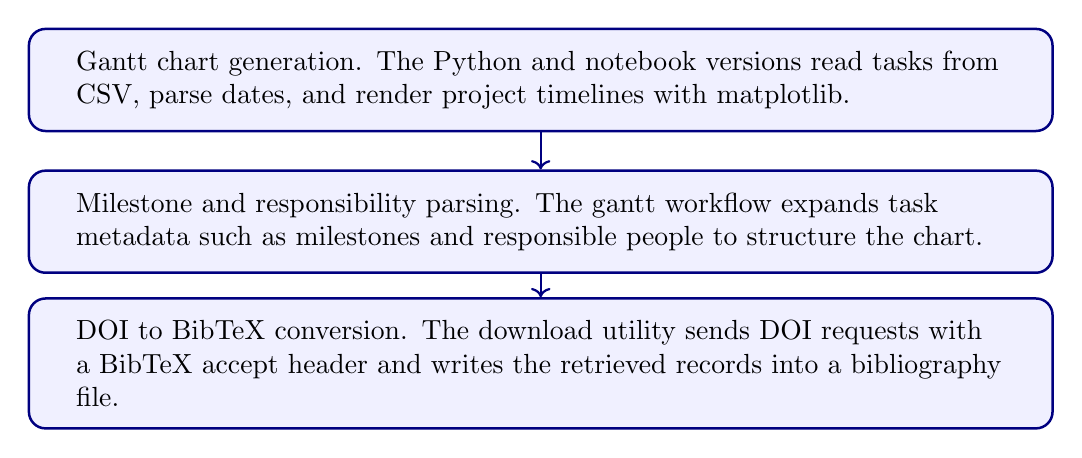
\begin{tikzpicture}[x=1cm,y=1cm]
    \node[methodbox] (m0) at (0,0.0) {Gantt chart generation. The Python and notebook versions read tasks from CSV, parse dates, and render project timelines with matplotlib.};
    \node[methodbox] (m1) at (0,-1.8) {Milestone and responsibility parsing. The gantt workflow expands task metadata such as milestones and responsible people to structure the chart.};
    \node[methodbox] (m2) at (0,-3.6) {DOI to BibTeX conversion. The download utility sends DOI requests with a BibTeX accept header and writes the retrieved records into a bibliography file.};
    \draw[->, thick, color=blue!50!black] (m0.south) -- (m1.north);
    \draw[->, thick, color=blue!50!black] (m1.south) -- (m2.north);
    \end{tikzpicture}
    \caption{Conceptual scheme for the methods in the productivityTools folder.}
    \label{fig:summary}
    \end{figure}

    
\bibliographystyle{plain}
\bibliography{../references}

\section*{Disclaimer}
These documents were generated with the assistance of ChatGPT 5.4. The material has been reviewed by the author before inclusion in this repository, but it is not free from possible errors.

\end{document}